\chapter{Foundations}
\label{foundations}
\section{Information Retrieval - Ranking Text}
\label{sec:ir}
Ranking is an integral part of the information retrieval (IR) process. The general IR problem can be formulated as follows: A user with a need for information expresses this information need through formulation of a query. Now given the query and a collection of documents, the IR system's task is to provide a list of documents that satisfy the user's information need. Furthermore, the retrieved documents should be sorted by relevance with respect to the user's query in descending order, i.e. the documents considered most relevant should be at the top of the list.

While given this formulation the task might appear simple at first, there are several caveats to look out for when it comes to ranking. For instance, there is no restriction on the structure of the query. While we might expect a natural language question like "What color are giraffes?" a user might decide to enter a keyword query like "giraffes color". The same applies to documents: Depending on the corpus we are dealing with, the documents might be raw text, structured text like HTML or even another type of media e.g. image, audio or a combination thereof.

Another possible issue is a mismatch between information need of the user and the corresponding query. Even if we find a perfect ordering of documents with respect to the query, we can not know for certain that the query actually reflects the user's information need. The user might not even know exactly what they're looking for until discovery through an iterative process, i.e. the information need is fuzzy and can not be defined by a single query from the start.

Furthermore, a query might require additional contextual information in order for an IR system to find relevant documents. For example, depending on the time at which a query is prompted, the correct answer might change: "Who is the president?" should return a different set of documents as soon as a new president has been elected. Also, since not specified further, it is up to interpretation what country's president the user is interested in. This also shows that some queries might depend on the user's location, i.e. the user might be interested in the president in their respective country.

In addition, the corpus might not be static either and change or grow over time. For example, web search has to deal with an ever-growing corpus: the Internet.

While this list of issues is not comprehensive, at this point the complexity of the ranking problem should have become apparent. Because this work focuses on the ranking of text in the context of web search, we will now give a formal definition with that scenario in mind:

Given a set of $|Q|$ natural language queries $Q = \{q_i\}_{i=1}^{|Q|}$ and a collection of $|D|$ documents $D = \{d_i\}_{i=1}^{|D|}$, we want to find a scoring function $s: Q \times D \rightarrow \R$, such that for any query $q \in Q$ and documents $d, d' \in D$, it holds true that $s(q, d) > s(q, d')$ if $d$ is more relevant w.r.t $q$ than $d'$.

To give the reader a more concrete idea and as we are going to build upon it throughout this thesis, we will now discuss two traditional approaches to text retrieval which, unlike neural IR, are based on exact matching, meaning query and document terms are compared directly. Moreover, they're "bag of word" models, meaning queries and documents are treated as sets of terms without considering order.

\subsection{TF-IDF}
Term Frequency - Inverted Document Frequency weighting (TF-IDF), is a traditional ranking approach that, given a query, assigns a relevance score to each document based on two assumptions:
\begin{enumerate}
    \item A document is relevant if terms from the query appear in it often.
    \item A document is relevant if the terms shared with the query are also rare in the collection.
\end{enumerate}

From these assumptions, two metrics are derived:
\begin{enumerate}
    \item Term-Frequency
          \begin{equation}
              w_{t,d} = \begin{cases}
                  1 + \log \tx{tf}_{t, d} & \tx{if } \tx{tf}_{t, d} > 0 \\
                  0                       & \tx{otherwise}              \\
              \end{cases}
          \end{equation}

          where $\tx{tf}_{t, d}$ is the count of term $t$ in document $d$. The logarithmic scaling is motivated by the idea that a document does not linearly become more relevant by the number of terms in it: A document containing a term 10 times more often doesn't necessarily mean it is $10$ times more important, e.g. the document might just be very long and contain more words in general. Note that this is just one possible normalization scheme out of many.

    \item Inverted Document Frequency
          \begin{equation}
              \tx{idf}(t, d) = \log \frac{|D|}{\tx{df}_t}
          \end{equation}
          where $\tx{df}_t$ counts the number of documents that a term occurs in over the full corpus. This way, terms that occur less frequently relative to the corpus size will receive a higher IDF score and those that are more frequent will receive a lower score.

\end{enumerate}

\begin{table}

\end{table}
To compute TF-IDF we can simply sum over the product of TF and IDF for each term in the query to produce a relevance score:
\begin{equation}
    \tx{score}(q, d) = \sum_{t \in q} w_{t,d} \times \tx{idf}_t
\end{equation}

\subsection{BM25}
\label{sec:bm25}
BM25 builds on the TF-IDF scores  by introducing additional hyperparameters and accounting for document length through a normalization term \citep{robertson2009probabilistic}. That way, short documents are preferred over long documents, if both have the same term frequency.

\begin{equation}
    \text{bm25}_{t,d} = \tx{idf}_t \frac{w_{t,d}}{k_1 \big((1 - b) + b \frac{\tx{len}(d)}{\tx{avglen}}\big) + w_{t,d}}
\end{equation}
Here, the free parameters $k_1$ and $b$ determine the how quick the bm25 function saturates with increasing term frequency (typically, $k_1=1.2$) and the degree to which document length affects the score, respectively. $\tx{len}(d)$ is the length of $d$ and \tx{avglen} the average document length over the corpus.

\section{Machine Learning}
\label{sec:ml}
Machine learning (ML) encompasses a set of statistical methods for automatically recognizing and extracting patterns from data. Typically, we can distinguish between two main types of machine learning: Supervised learning and unsupervised learning.

In the case of supervised learning, we have a set of training instances $X = \{x_i\}_{i=1}^N$ and corresponding labels $Y = \{y_i\}_{i=1}^N$, assigning a certain characteristic to each data point. For example, this characteristic might be a probability distribution over a set of classes or a regression score. If each $y_i$ represents one or more categories from a fixed set of classes $C = \{c_i\}_{i=1}^{|C|}$, it is called a classification problem.

Now given the training data and labels, the goal is to find a hypothesis that explains this data, such that for unseen data points $x' \notin X$, the labels $y' \notin Y$ can be inferred automatically. One way to estimate the generalization ability of a model or algorithm is to divide the dataset into a training and a test set, and only train on the training set while using the test set for evaluation. If the test set models the full distribution of data adequately, it may act as a proxy for estimating the error on unseen samples.

In contrast, when performing unsupervised learning there is no access to any labels whatsoever. Characteristics of the data need to be learned solely from the data $X$ itself. Examples for this include clustering where $X$ is clustered into groups, representation learning which usually tries to find vector representations for $X$, as well as dimensionality reduction which, if each $X$ is already a vector, tries to compress them into more compact but still informative representations.

That being said, the lines separating supervised and unsupervised learning have become blurry. Especially with the emergence of semi-supervised approaches and "end2end" representation learning, modern ML methods often integrate parts of both.

\section{Deep Learning}
\label{sec:dl}
Deep learning is a subfield of ML that makes use of a class of models called Deep Neural Networks (DNN). Typically, DNNs find application in the supervised learning scenario and are often used for classification tasks. In the following we explain the basic mechanisms of DNNs and common approaches to train them.

\subsection{Deep Neural Networks}
In essence, a Deep Neural Network (DNN) is a function approximator $f: \R^n \rightarrow \R^m$ that applies a series of non-linear transformations to its inputs in order to produce an output. In its simplest form, an input vector $x \in \R^n$ is multiplied by a single weight matrix, a bias vector is added, and the resulting vector is passed through a non-linear activation function $\sigma$:

\begin{equation}
    f(x) = \sigma(W x + b)
\end{equation}
where $W \in \R^{m \times n}$ and $b \in \R^{m}$ are learnable parameters.
This model is commonly referred to as single layer feed-forward neural network (FFN) or single layer perceptron.

When used for classification, a single layer FFN is limited to problems that solely require linear separation in order to be solved. To learn more complex, non-linear decision boundaries, multiple layers can be applied in sequence.

An $L$-layer DNN can be described as follows:

\begin{equation}
    \label{eq:DNN}
    \begin{split}
        h^{(1)} &= \sigma^{(1)}(W^{(1)} x + b^{(1)}) \\
        h^{(2)} &= \sigma^{(2)}(W^{(2)} h^{(1)} + b^{(2)}) \\
        & \vdots \\
        f(x) &= \sigma^{(L)}(W^{(L)} h^{(L-1)} + b^{(L)})
    \end{split}
\end{equation}
Common choices for $\sigma$ include:

\begin{itemize}
    \item $\sigma(x) = \frac{1}{1 + e^{-x}}$ (sigmoid)
    \item $\tanh(x) = \frac{e^x - e^{-x}}{e^x + e^{-x}}$ (hyperbolic tangent)
    \item $\text{softmax}(x_i) = \frac{e^{x_i}}{\sum_j e^{x_j}}$ (softmax)
    \item $\text{ReLU}(x) = \max(0, x)$ (rectified linear unit \citep{nair2010rectified})
\end{itemize}

\subsection{Optimization}
Arguably, the most common way for optimizing a neural network are the gradient descent (GD) algorithm and its variants. For this, an objective function $J(\theta)$ is defined, based on the DNN's outputs and corresponding target labels over the training set.

\begin{equation}
    J(\theta) = \frac{1}{N} \sum_{i=1}^{N} \mathcal{L}(f(x_i; \theta), y_i)
\end{equation}
Here, $\mathcal{L}$ is a differentiable loss function and $\theta$ represents the vector of all learnable parameters of the neural network $f(x)$.

\subsubsection{Gradient Descent}
For GD, the gradient of $J(\theta)$ with respect to $\theta$ is computed and scaled by a hyperparameter called learning rate $\eta$. If the objective is to minimize, the scaled gradient is subtracted from the original parameter vector.

\begin{equation}
    \theta_{new} = \theta - \eta\nabla_\theta J(\theta)
\end{equation}
By repeating this procedure iteratively, we can gradually minimize $J(\theta)$. Common choices for $\mathcal{L}$ include:
\begin{itemize}
    \item \textbf{Cross Entropy Loss}
          \begin{equation}
              \label{eq:ce_loss}
              \tx{CE}(y, \hat{y}) = - \sum_{k=1}^C y_k \log \hat{y}_k
          \end{equation}
          For classification tasks, where $y_k$ is the ground truth probability of class $k$ and $\hat{y}_k$ the corresponding prediction.

    \item \textbf{Mean Squared Error}
          \begin{equation}
              \tx{MSE}(y, \hat{y}) = (y - \hat{y})^2
          \end{equation}
          In the case of regression.
\end{itemize}

\subsubsection{Stochastic Gradient Descent}
The aforementioned algorithm is also known as the batch gradient descent (BGD) variant. Stochastic Gradient Descent (SGD) differs from BGD in the number of training samples that are used for a gradient update. Where BGD uses the gradient of the full training set for updating $\theta$, SGD only considers a single, randomly picked sample for each update. Not only can this approach be more efficient, since fewer redundant computations are performed, due to its stochastic nature it is also more likely to break out of local minima, allowing additional exploration for better solutions \citep{ruder2016overview}.

\subsubsection{Mini-Batch Gradient Descent}
While SGD's high variance during training makes it more likely to escape local minima, it can also come with the disadvantage of unstable training. In this scenario, convergence might be hindered by overshooting desirable minima.

To mitigate this issue, we can simply use more than one sample in order to achieve a more accurate estimate of the full gradient. Now, at each step a small subset of the dataset is sampled to reduce variance and stabilize training while retaining a level of stochasticity. This variant of gradient descent is called mini-batch gradient descent.

Building on mini-batch GD, many algorithms have been introduced in the context of DNNs, which employ further optimizations in order to improve convergence speed and quality. Notable examples include:
\begin{itemize}
    \item Adagrad \citep{duchi2011adaptive}
    \item RMSProp \citep{hinton2012neural}
    \item Adam \citep{kingma2014adam}
\end{itemize}

\begin{algorithm}
    \SetAlgoLined
    \KwData{$X=\{(x_0, y_0), ..., (x_n, y_n)\}$ training examples and target labels.}
    \KwIn{function $f$ with trainable parameters $\theta$}
    initialize $\theta$ with random values \;
    \While{not converged}{
    $B \leftarrow \tx{next k training pairs} \in X$ \;
    $\theta \leftarrow \theta - \eta\nabla_\theta\big(\frac{1}{k} \sum_{(x_i, y_i) \in B}\mathcal{L}(f(x_i; \theta), y_i)\big)$ \;
    }
    \caption{Mini-Batch Gradient Descent with batch size $k$, learning rate $\eta$}
\end{algorithm}

\subsubsection{Backpropagation}
\label{sec:backprop}
Because a neural network may consist of multiple layers and therefore, is a composition of multiple non-linear functions, computing the gradient w.r.t. each parameter of the network can become a non-trivial and even cumbersome task, if done by hand. One popular way of automatically computing the gradients of a DNN is the backpropagation algorithm \citep{rumelhart1988learning}.

Backpropagation is a direct application of the chain rule for calculating the derivative of the composition of two functions. Given two differentiable functions $f(x)$ and $g(x)$, the chain rule states that the derivate of their composition $f(g(x))$ is equal to the partial derivative of $f$ w.r.t. $g$, times the partial derivate of $g$ w.r.t. $x$.

\begin{equation}
    \frac{\partial f(g(x))}{\partial x} = \frac{\partial f(g(x))}{\partial g(x)} \frac{\partial g(x)}{\partial x}
\end{equation}
Let $a^{(k)} = W^{(k)} h^{(k-1)} + b^{(k)}$ be the intermediate output of an $L$-layer DNN at layer $k$, before passing it through an activation function $\sigma$ (See \ref{eq:DNN}). With a single application of the chain rule we can compute the gradient of the objective function $J$ w.r.t. $a^{(L)}$ like so:

\begin{equation}
    \frac{\partial J}{\partial a^{(L)}} = \frac{\partial J}{\partial \sigma(a^{(L)})} \frac{\partial \sigma(a^{(L)})}{\partial a^{(L)}}
\end{equation}
If we now apply the chain rule a second time, we can produce a term for computing the derivative w.r.t. $W^{(L)}$.

\begin{equation}
    \frac{\partial J}{\partial W^{(L)}} = \frac{\partial J}{\partial \sigma(a^{(L)})} \frac{\partial \sigma(a^{(L)})}{\partial a^{(L)}} \frac{\partial a^{(L)}}{W^{(L)}}
\end{equation}
Note that we now only need to know the derivatives of $J$, $\sigma$ and $a^{(L)}$ separately, in order to compute the derivative of their composition. By recursively applying this rule, we can compute partial derivatives of $J$ w.r.t. parameters of the DNN, up to an arbitrary depth, as long as all functions it is composed of are differentiable.

By modeling the chain of operations in a DNN as a computation graph, deep learning frameworks like PyTorch \citep{NEURIPS2019_9015} or Tensorflow \citep{tensorflow2015-whitepaper} are capable of automatically performing backpropagation, as long as each operation's derivative is known and pre-defined in the library.

\subsection{Regularization}
Regularization includes a number of techniques to improve the generalization capabilities of an ML model. If an ML model achieves a low error rate on training data but a high error rate on test data, it is said to be \ti{overfitting}. In this scenario, the model has essentially "memorized" the training data and can no longer adapt to unseen examples. Regularization techniques tackle this problem by limiting the hypothesis space of models through favoring simple solutions over complex ones.

\subsubsection{Weight Decay}
Weight decay constraints the number of possible hypothesis by adding a penalty based on model parameters. For example, L2-regularization encourages small weights that lie on a hypersphere by adding the sum of squares over all parameters to the loss function.

\begin{equation}
    J(\theta) = \mathcal{L}(\theta) + \lambda ||\theta||_2^2
\end{equation}
As L2 is only a soft constraint, its effect can be regulated by hyperparameter $\lambda$.

\subsubsection{Dropout}
Dropout is a DNN specific method that, during training time, randomly sets entries in the input vector of a layer to $0$ with probability $p$ \citep{DBLP:journals/corr/abs-1207-0580}. The initial idea of this approach is to prevent groups of neurons from co-adapting, i.e. requiring the activation of one another in order to detect a certain feature. If dropout is employed, a neuron can no longer rely on the presence of another neuron. Dropout can also be interpreted as a way of training an ensemble of sub-networks of the original network which share the same parameters.


\section{Transformer Models}
\label{sec:transformer}
One of the most prominent deep learning architectures of the past years is the transformer \citep{vaswani2017attention}. The transformer and its variants have set multiple state-of-the-art records in a variety of NLP tasks \citep{devlin-etal-2019-bert, DBLP:journals/corr/abs-1907-11692, DBLP:journals/corr/abs-2003-10555, DBLP:journals/corr/abs-1909-08053, DBLP:journals/corr/abs-2005-14165}, and have since been adapted to other domains such as computer vision \citep{DBLP:journals/corr/abs-2010-11929} or audio generation \citep{https://doi.org/10.48550/arxiv.2005.00341}.

Unlike previous methods for embedding words in vector spaces, which relied on word co-occurrence to learn a single fixed vector for each token \citep{pennington2014glove, DBLP:journals/corr/abs-1301-3781}, transformers are able to produce \ti{contextualized} word embeddings. This means that the representation of each word in a sequence changes dynamically based on its context, i.e. all other words in the sequence.

In this section we will discuss the architecture and ideas behind it and explain one of the most popular training approaches for NLP, named BERT \citep{devlin-etal-2019-bert}.

\subsection{Architecture}
The transformer architecture is based on a single building block which, after an input layer, is repeatedly applied in order to form the full model. Throughout this thesis we will also refer to these building blocks as layers, e.g. a $12$-layer model consists of an input layer followed by $12$ blocks. A single transformer block consists of:
\begin{itemize}
    \item a multi-head attention layer
    \item a point-wise feed-forward layer
    \item residual connections
    \item layer normalization
\end{itemize}
We will first explain the input layer, then go over each of these elements and explain how a transformer block is constructed from them.


\subsection{Input Layer}
The transformer's input layer takes in a sequence of tokens and produces continuous representations by selecting corresponding vectors from a learned embedding matrix $M \in \R^{d \times |V|}$. Here $|V|$ denotes the size of the vocabulary and $d$ the hidden dimension of the model. Because the transformer model itself does not encode the order of its inputs, \ti{positional encodings} are added to the initial embeddings for injecting positional information.

One way for generating positional encodings is to introduce a new set of learned embeddings of dimension $d$, one for each input position. However, this approach requires a fixed maximum input length, as all embeddings have to be defined before training. Alternatively, \citep{vaswani2017attention} propose to use sine and cosine waves as a function of the position:

\begin{equation}
    \text{PE}_{(pos, 2i)} = \sin\bigg(\frac{pos}{10000^{\frac{2i}{d}}}\bigg)
\end{equation}
\begin{equation}
    \text{PE}_{(pos, 2i + 1)} = \cos\bigg(\frac{pos}{10000^{\frac{2i}{d}}}\bigg)
\end{equation}
where $pos$ and $i$ denote position along sequence and hidden dimension respectively. In terms of machine translation, they've found this approach to perform nearly identical to learned embeddings.

\subsection{Multi-Head Self-Attention}
\subsubsection{The Attention Mechanism}
Originally, attention mechanisms have been proposed in the context of neural machine translation (NMT) \citep{bahdanau2014neural,luong2015effective}. Particularly, they were used for aligning words from a source language with their corresponding translations, i.e. pointing out the source words that are relevant for predicting the next translation target. The alignment is important, as different languages usually do not share the same word order, making a sequential word-to-word translation infeasible.

Generally speaking, attention is a mechanism that allows a model to focus on parts of its inputs, usually while considering a certain context. This could for example be words in a text (inputs) that are regarded important for answering a question (context) \citep{xiong2016dynamic} or patches of pixels in an image (inputs) that are important for detecting a certain object type (context) \citep{xu2015show}.

Given a sequence of $N$ input vectors $X = (x_1, \dots, x_N) \in \R^{N \times d}$ and $M$ context vectors $C = (c_1, \dots, c_M) \in \R^{M \times d}$, we can describe the general attention mechanism as follows:

\begin{align}
     & s_{ij} = a(x_i, c_j)                                         \\
     & \alpha_{ij} = \frac{\exp(s_{ij})}{\sum_{k=1}^N \exp(s_{kj})} \\
     & h_j = \sum_{k=1}^N \alpha_{kj} x_k
\end{align}
where $a: \R^d \times \R^d \rightarrow \R$ is a scoring function that assigns importance scores to input $x_i$ given context $c_j$. The attention weights $\alpha_{ij}$ are then used to produce a context-sensitive representation $h_j$ as weighted sum over $X$.

Common choices for $a$ include:
\begin{itemize}
    \item $a(u, v) = u \cdot v$ (dot product)
    \item $a(u, v) = w^\top \tanh(W u + U v)$ (additive)
    \item $a(u, v) = \sigma(w^\top \tanh(W u + U v + b) + c)$ (MLP)
\end{itemize}

\subsubsection{Self-Attention}
Self-Attention is a special case of attention where input vectors and context vectors stem from the same input sequence. It can be seen as the model attending to a sequence, given the sequence itself as context. In \citep{vaswani2017attention} a third set of \ti{value} vectors is introduced, resulting in three sequences termed \ti{query}, \ti{key} and \ti{value} vectors, in analogy to memory lookups.

To produce these vectors, the initial input sequence is transformed by three different learned weight matrices, namely $W^{(q)}, W^{(k)} \in \R^{d \times d_k}$ and $W^{(v)} \in \R^{d \times d_v}$.

\begin{align}
    Q & = X W^{(q)} \\
    K & = X W^{(k)} \\
    V & = X W^{(v)}
\end{align}
Then, using the obtained query and key vectors $Q$ and $K$, a matrix of attention scores is computed and matrix multiplied with $V$:

\begin{equation}
    \text{SelfAttention}(Q, K, V) = \text{softmax}\bigg(\frac{Q K^\top}{\sqrt{d_k}}\bigg) V
\end{equation}
As a consequence, each vector in the resulting sequence becomes an attention weighted sum over the vectors in $V$. Note the scaling by $\sqrt{d_k}$, which is supposed to prevent oversaturation of the softmax function due to large dot-products.

From the memory lookup perspective: Query vectors $Q$ are matched with key vectors $K$, in order to produce compatibility scores. These scores are then used to retrieve value vectors from $V$ via soft-lookup.

\subsubsection{Multi-Head Attention}
Self-Attention can further be extended to multi-head attention by running multiple self-attention layers in parallel, then concatenating and projecting their outputs:
\begin{equation}
    \tx{MultiHeadAttention}(Q, K, V) = \bigg[ \bigparallel_{i=1}^h \tx{SelfAttention}_i(Q,K,V) \bigg] W\lay o
\end{equation}
where $h$ is the number of attention-heads, $||$ denotes concatenation and $W\lay o \in \R^{d_v h \times d}$ is a learned matrix for projecting back to the model's original hidden dimension.

Note that in the default case, each attention layer has its own weight matrices. However,  we omit layer indices to keep the notation more simple.

\subsection{Point-wise Feed-forward}
The point-wise feed-forward component is a 2-layer MLP that is applied to each position along the sequence dimension, meaning weight parameters are shared across all positions. It follows the following architecture:
\begin{equation}
    \tx{FFN}(x) = \tx{ReLU}(x W^{(0)} + b^{(0)}) W^{(1)} + b^{(1)}
\end{equation}

\subsection{Residual Connection}
After applying a layer or block of layers in a DNN, if we add the inputs back to its outputs, we introduce a residual connection or skip connection:

\begin{equation}
    \tx{Residual}(x) = f^{(k)}(x) + x
\end{equation}
where $f^{(k)}(x)$ is the layer at depth $k$.

The most prominent motivation for residual connections is that they facilitate the training of deeper neural networks. A common issue with deep neural networks is the vanishing gradient problem. As computing gradients through backpropagation relies on a series of multiplications of potentially small values (\Cref{sec:backprop}), gradients tend to become smaller the further we propagate back. This makes training very deep networks harder, as early layers might receive little to no updates.

Since $\tx{residual}'(x) = f'(x) + 1$, the gradient of the residual connection will be $>~1$, even if the gradient is $<1$, alleviating the effect of vanishing gradients. It can also be interpreted as preserving more of the initial input information throughout the network, treating the DNN layers as an addition to the identity function instead of a full transformation of the input.

% vanishing gradients
% identity function idk read up
% improve gradient flow for deep models
\subsection{Layer Normalization}
Layer Normalization \citep{ba2016layer} is another technique for training deeper neural networks. When training machine learning models on numerical features, it is common practice to normalize inputs, e.g. such that their distribution is centered at $0$ and has a standard deviation of $1$. This way, there's less variance across features, resulting in more stable training and hence improving convergence.

However, since DNNs pass features through multiple layers, there's no guarantee that hidden representations will maintain a reasonable scale, meaning each layer might have to adapt to a new distribution \citep{DBLP:journals/corr/IoffeS15}. Layer Normalization tackles this problem by computing mean $\mu^{(k)}$ and standard deviation $\sigma^{(k)}$ over the feature dimension of each hidden layer $k$:

\begin{equation}
    \mu\lay k = \frac{1}{d} \sum_{i=1}^d z_i\lay k
\end{equation}

\begin{equation}
    \sigma^{(k)} = \sqrt{\frac{1}{d} \sum_{i=1}^d (z_i^{(k)} - \mu^{(k)})^2}
\end{equation}
here $z_i^{(k)}$ denotes the $i$-th output of layer $k$ with hidden dimension $d$, before applying an activation function.\\
These layer statistics are then used to normalize the hidden layer representation $z^{(k)}$:

\begin{equation}
    \tx{LayerNorm}(z\lay k) = \gamma \lay k \circ \frac{z\lay k - \mu\lay k}{\sigma\lay k} + \beta\lay k
\end{equation}
where $\gamma^{(k)}$ and $\beta^{(k)}$ are learned parameter vectors for layer $k$ and $\circ$ denotes the element-wise product. Further, $\gamma^{(k)}$ and $\beta^{(k)}$ are additional learnable parameters for adjusting scale and shift of the normalized distribution if required.

\subsection{The Full Transformer Block}

The full transformer block can be described with the following equations:

\begin{align}
    A              & = \tx{MultiHeadAttention}(X, X, X) \\
    Z              & = \tx{LayerNorm}(A + X)            \\
    \tx{TBlock}(X) & = \tx{LayerNorm}(\tx{FFN}(Z) + Z)
\end{align}
It consists of a multi-head attention layer and a point-wise fully connected layer, each followed by residual connection and layer normalization.

\begin{figure}[h]
    \centering
    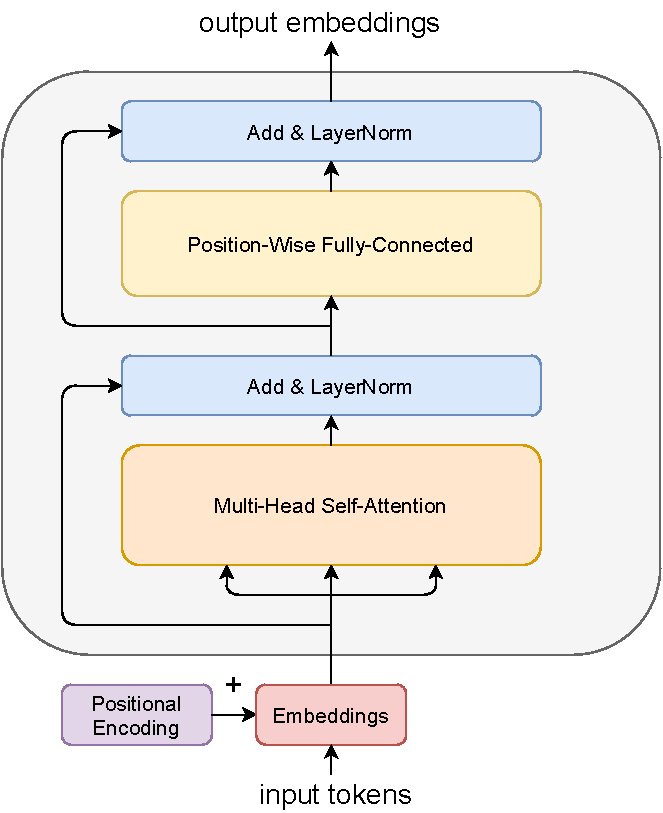
\includegraphics[width=0.6\textwidth]{gfx/transformer}
    \caption{Schematic overview of the transformer block and the transformer's input layer at the bottom.}
\end{figure}


\subsection{BERT Pre-Training}
A key part leading to the success of transformer models is their effectiveness in large-scale transfer learning. In the context of NLP, the transfer learning procedure typically consists of two stages: First, a model is pre-trained on large amounts of human generated text data (e.g. from the Internet), using language modeling as an objective. Then, the model is fine-tuned on a downstream task for which only limited amounts of data are available. As the model has already learned basic language concepts during pre-training, it can now leverage this knowledge for the new task instead of learning it from scratch.

One particular approach to transfer learning for transformers, which has pushed the state-of-the-art on several NLP benchmarks, is BERT (Bidirectional Encoder Representations from Transformers) \citep{devlin-etal-2019-bert}. Unlike previous pre-training approaches that optimized for traditional \ti{left-to-right} language modeling \citep{DBLP:journals/corr/abs-1801-06146,Peters:2018,radford2018improving}, BERT employs a bidirectional objective.

In left-to-right language modeling the goal is to predict the next word in a sequence of words, given the preceding words. BERT on the other hand employs a \ti{masked language model} (MLM) objective. Here, tokens from the input sequence are randomly masked out or replaced with random tokens. The model then has to predict what the actual token should be.

This means that, during pre-training, traditional language models only have access to the context left to their current prediction, while BERT has access to context in both directions.

In addition to MLM, BERT introduces a \ti{next-sentence prediction} (NSP) task where, given two sentences, the model has to determine whether the second sentence follows the first, or was selected randomly. This is motivated by language tasks often requiring to model the relation between two sentences.

While many improved training procedures have been proposed since BERT, which often replace NSP or introduce additional objectives \citep{DBLP:journals/corr/abs-2003-10555, DBLP:journals/corr/abs-1907-11692, 10.5555/3454287.3454804, Lan2020ALBERT}, MLM still remains as an integral part for most approaches.

\section{Probing}
Probing is a method for estimating the presence of certain properties in dense vector representations of neural network models. For this, a classifier (\ti{probe}) $P$ is trained on the fixed representations of a \ti{subject model} $\mathcal{M}$, to predict property $Y$. In NLP we typically probe for linguistic properties in word embeddings. For example, we could estimate the presence of part-of-speech (POS) information by predicting POS tags. Based on the probe's performance, e.g. when compared to embeddings from a random baseline, we can conclude whether the property can be decoded from the subject model's representations.